\documentclass[10pt]{article}
\usepackage[margin=0.8in]{geometry}
\usepackage[utf8]{inputenc}
\usepackage[T1]{fontenc}
\usepackage[english]{babel}

\usepackage{fourier}
\usepackage{amsmath}
\usepackage{amssymb}
\usepackage{amsfonts}
\usepackage{amsthm}

\usepackage{graphicx}
\usepackage{float}
\usepackage{caption}
\usepackage{subcaption}
\usepackage{adjustbox} % Good for image handling

\usepackage{booktabs}

\usepackage{etoolbox}
\usepackage{siunitx}
\usepackage{parskip} % Creates space between paragraphs instead of indentation
\setlength{\parskip}{1em} % Adjust space between paragraphs
\setlength{\parindent}{0pt} % No indentation

\usepackage{tikz} % For diagrams
\usetikzlibrary{shapes.geometric, arrows, positioning}

\usepackage{hyperref}
\hypersetup{
    colorlinks=true,
    linkcolor=blue,
    filecolor=magenta,
    urlcolor=cyan,
}
\usepackage{cite}

\usepackage{listings}
\usepackage{color}

\definecolor{codegreen}{rgb}{0,0.6,0}
\definecolor{codegray}{rgb}{0.5,0.5,0.5}
\definecolor{codepurple}{rgb}{0.58,0,0.82}
\definecolor{backcolour}{rgb}{0.95,0.95,0.92}

\lstdefinestyle{mystyle}{
    backgroundcolor=\color{backcolour},
    commentstyle=\color{codegreen},
    keywordstyle=\color{magenta},
    numberstyle=\tiny\color{codegray},
    stringstyle=\color{codepurple},
    basicstyle=\ttfamily\footnotesize,
    breakatwhitespace=false,
    breaklines=true,
    captionpos=b,
    keepspaces=true,
    numbers=left,
    numbersep=5pt,
    showspaces=false,
    showstringspaces=false,
    showtabs=false,
    tabsize=2,
    language=C++
}
\lstset{style=mystyle}

\newcommand{\code}[1]{\texttt{#1}}


\title{Assignment 4: Hybrid MPI + FastFlow MergeSort}
\author{Luca Lombardo \\ SPM Course a.a. 24/25}
\date{}

\begin{document}

\maketitle
\vspace{-1.5em} % Reduce space after title block


The goal of this project was to develop a scalable MergeSort algorithm for a large array of records, combining intra-node parallelism with FastFlow and inter-node parallelism with MPI.
\section{Implementation Strategy}

At the outset, a key design decision was made regarding the \code{Record} data structure. While the assignment specified a fixed-size payload array (\code{char rpayload[RPAYLOAD]}), we opted for a more flexible structure with a dynamically allocated payload (\code{char* payload}). This choice was motivated by the need for a versatile and robust benchmarking framework. Using a dynamic payload allows the record size to be configured at runtime via command-line arguments, which is essential for systematic performance analysis across various payload sizes without requiring code recompilation for each test. This design choice does not compromise the performance analysis. The memory for each record's payload is allocated once at the beginning of the tests and remains fixed throughout the sorting process. Within the core sorting algorithms, the cost of moving or comparing these records is dominated by the size of the payload, not by the fact that it is heap-allocated. The use of move semantics in our data structures ensures that during merge operations, only the pointer and size are transferred, not the payload data itself, preserving performance characteristics equivalent to those of a fixed-size struct for the purpose of this study.



\subsection{Single-Node Parallel Design (FastFlow)}
For the shared-memory implementation, we adopted a pragmatic, performance-oriented approach. The MergeSort algorithm naturally decomposes into two distinct phases: an initial, highly parallel sorting of small data chunks, followed by a sequential series of merge passes. Our implementation mirrors this structure, using dedicated FastFlow farms for each phase to maximize performance.

\textbf{Phase 1: Parallel Sorting.} The first challenge is to break down the massive initial array into manageable pieces. We split the array into numerous small, cache-friendly chunks. The sorting of these chunks is an embarrassingly parallel problem. For this task, we employed an \code{ff\_farm}. An emitter node decomposes the array into tasks, and a pool of worker threads processes them concurrently. Each worker sorts its assigned chunk in-place using \code{std::sort}, which is highly optimized for small-to-medium datasets.

\textbf{Phase 2: Iterative Merging.} Once the initial chunks are sorted, they must be progressively merged. This is an inherently iterative process. We implemented this using a loop where, at each iteration, a new \code{ff\_farm} is created to perform a single merge pass in parallel. In each pass, pairs of adjacent sorted runs are merged into a new, larger sorted run. A critical optimization here is the use of a "ping-pong" buffer strategy. We allocate a single auxiliary buffer of the same size as the original data. In each merge pass, we read from a source buffer and write the merged results to a destination buffer. After the pass is complete, we simply swap the pointers, so the destination becomes the source for the next iteration. This avoids costly data copies between passes and is a standard, highly efficient technique for out-of-place merge algorithms.

\subsubsection{Architectural Considerations and Discarded Alternatives}
The assignment suggested exploring FastFlow's building blocks, including \code{ff\_pipeline} and \code{ff\_all2all}. We implemented and evaluated these alternatives but ultimately discarded them for sound performance and algorithmic reasons.

\textbf{Why not \code{ff\_all2all}?} The \code{ff\_all2all} pattern is designed for data redistribution, where each worker sends a piece of its local data to every other worker. This is the core of algorithms like Radix Sort or Sample Sort, which partition data based on key values. MergeSort, however, relies on merging physically adjacent, sorted segments. Its communication pattern is strictly pairwise and hierarchical, not all-to-all. Forcing MergeSort into an all-to-all pattern would be algorithmically incorrect.

\textbf{Why not \code{ff\_pipeline}?} An integrated pipeline architecture, such as \code{feeder -> sort\_stage -> merge\_stage}, seems theoretically elegant. We invested significant effort in implementing and benchmarking this alternative. However, it yielded a significant performance degradation, reducing the peak speedup of about 30\%. This counter-intuitive result stems from two main factors.
First, MergeSort is fundamentally a bulk-synchronous parallel (BSP) algorithm: the merge phase cannot begin until the entire sort phase is complete. There is no opportunity for true, overlapping pipelining.
Second, the \code{ff\_pipeline} introduces communication and scheduling overhead between its stages. For a single, large task traversing the pipeline, this overhead outweighs any potential benefits, especially when compared to the lean approach of dedicating all parallel resources to a single, optimized farm for each distinct phase. We therefore concluded that the architecturally simpler two-farm approach was pragmatically superior for this specific problem.

\subsection{Hybrid Multi-Node Design (MPI + FastFlow)}
To scale the algorithm beyond a single node, we designed a hybrid implementation that uses MPI for inter-node coordination and our optimized FastFlow MergeSort for intra-node computation. The overall process is divided into three main phases.

\textbf{Phase 1: Data Distribution.} The root process (rank 0), holding the initial dataset, first partitions the global dataset into $P$ contiguous blocks, where $P$ is the number of MPI processes. The size of each block is calculated to ensure the workload is as balanced as possible. The root then uses \code{MPI\_Scatterv} to send each partition to its designated process. This is more robust than a simple \code{MPI\_Scatter} as it correctly handles cases where the total number of records is not perfectly divisible by $P$.

\textbf{Phase 2: Local Sorting.} Upon receiving its local data segment, each MPI process invokes the highly optimized, multi-threaded \code{parallel\_mergesort} function. This step agglomerates fine-grained comparison operations into a coarse-grained local sort, leveraging all available cores on the node. This phase is entirely computation-bound and transforms the global problem into a set of distributed, sorted arrays.

\textbf{Phase 3: Hierarchical Merging.} After the local sort, the distributed sorted segments must be merged into a single, globally sorted array at the root. We chose a binary tree reduction pattern for this task, as illustrated in Figure \ref{fig:mpi_merge_tree}. The merging occurs in $\log_2(P)$ steps. In each step, active processes are paired up: one "sender" sends its data to a "receiver". The receiver merges its own data with the incoming data, and the sender then becomes idle. This pattern distributes the merge work effectively across multiple nodes in the early stages.

A critical design decision in this phase concerned the communication strategy. The assignment suggested maximizing computation-to-communication overlap, which typically implies the use of non-blocking primitives like \code{MPI\_Irecv}. We thoroughly investigated this path and developed a prototype based on this pattern. However, our analysis and benchmarking led to a deliberate engineering choice to use a simpler, more robust model based on blocking communication (\code{MPI\_Recv}) for each merge step. This decision was based on two key findings. First, the MergeSort algorithm itself offers limited opportunities for meaningful overlap; the core merge logic cannot proceed until it has received the initial segments of data from its partner, making it difficult to hide communication latency behind computation. Second, the management of non-blocking requests within an iterative algorithm like the binary tree reduction introduced significant complexity and a measurable performance overhead that negated the theoretical benefits. Therefore, the final implementation prioritizes correctness and real-world performance over a theoretically optimal but practically less effective strategy.


\begin{figure}[H]
    \centering
    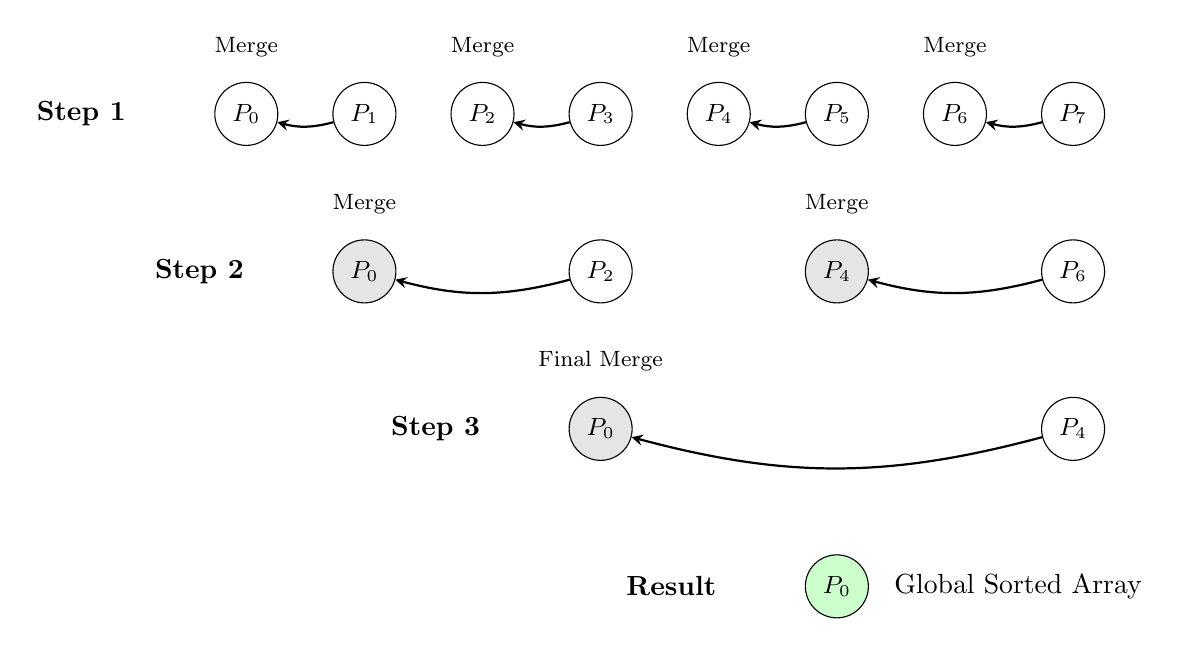
\begin{tikzpicture}[
            node distance=1.5cm and 0.8cm,
            proc/.style={circle, draw, minimum size=0.8cm, font=\small},
            arrow/.style={-stealth, thick}
        ]
        % Initial processes
        \foreach \i in {0,...,7} {
                \node[proc] (p\i) at (\i*1.5, 0) {$P_\i$};
            }

        % Step 1
        \draw[arrow] (p1) to[bend left=15] (p0);
        \draw[arrow] (p3) to[bend left=15] (p2);
        \draw[arrow] (p5) to[bend left=15] (p4);
        \draw[arrow] (p7) to[bend left=15] (p6);
        \node[above=0.2cm of p0, font=\footnotesize] {Merge};
        \node[above=0.2cm of p2, font=\footnotesize] {Merge};
        \node[above=0.2cm of p4, font=\footnotesize] {Merge};
        \node[above=0.2cm of p6, font=\footnotesize] {Merge};
        \node[left=1cm of p0, font=\bfseries] {Step 1};

        % Step 2
        \node[proc, fill=gray!20] (p0_2) at (1*1.5, -2) {$P_0$};
        \node[proc] (p2_2) at (3*1.5, -2) {$P_2$};
        \node[proc, fill=gray!20] (p4_2) at (5*1.5, -2) {$P_4$};
        \node[proc] (p6_2) at (7*1.5, -2) {$P_6$};
        \draw[arrow] (p2_2) to[bend left=15] (p0_2);
        \draw[arrow] (p6_2) to[bend left=15] (p4_2);
        \node[above=0.2cm of p0_2, font=\footnotesize] {Merge};
        \node[above=0.2cm of p4_2, font=\footnotesize] {Merge};
        \node[left=1cm of p0_2, font=\bfseries] {Step 2};

        % Step 3
        \node[proc, fill=gray!20] (p0_3) at (3*1.5, -4) {$P_0$};
        \node[proc] (p4_3) at (7*1.5, -4) {$P_4$};
        \draw[arrow] (p4_3) to[bend left=15] (p0_3);
        \node[above=0.2cm of p0_3, font=\footnotesize] {Final Merge};
        \node[left=1cm of p0_3, font=\bfseries] {Step 3};

        % Final result
        \node[proc, fill=green!20] (p0_final) at (5*1.5, -6) {$P_0$};
        \node[right=0.2cm of p0_final] {Global Sorted Array};
        \node[left=1cm of p0_final, font=\bfseries] {Result};
    \end{tikzpicture}
    \caption{Illustration of the 8-process binary tree merge reduction. Active merging processes are shown in gray, with the final result in green.}
    \label{fig:mpi_merge_tree}
\end{figure}

\subsubsection{Alternative Merge Strategy: Centralized K-Way Merge}
We also implemented and evaluated an alternative strategy for the final merge phase: a centralized k-way merge. In this model, all non-root processes ($P-1$ of them) send their locally sorted data directly to the root process in a single communication round. The root process then performs a k-way merge on all $P$ partitions (including its own) using a min-heap.

Theoretically, this approach is attractive as it reduces the number of communication rounds from $\log_2(P)$ to one. However, our benchmarks showed it to be less performant than the binary tree reduction. The primary reason is that it creates a massive bottleneck at the root process. The root must handle incoming network traffic from all other processes simultaneously while also performing the entire k-way merge. This serializes a large portion of the work and underutilizes the other nodes. In contrast, the binary tree approach distributes the merge workload across multiple nodes in the initial steps, leveraging the computational power of the entire system for longer before idling processes. The higher parallelism of the binary tree approach outweighed the benefit of fewer communication rounds for the problem scales tested.

\section{Performance Analysis}
We benchmarked our implementations to evaluate their strong and weak scaling properties. We define "absolute speedup" as the ratio between the execution time of the best sequential algorithm (\code{std::sort}) and our parallel implementation. The analysis is based on the data collected and visualized below.

\begin{figure}[H]
    \centering
    \begin{subfigure}{0.49\textwidth}
        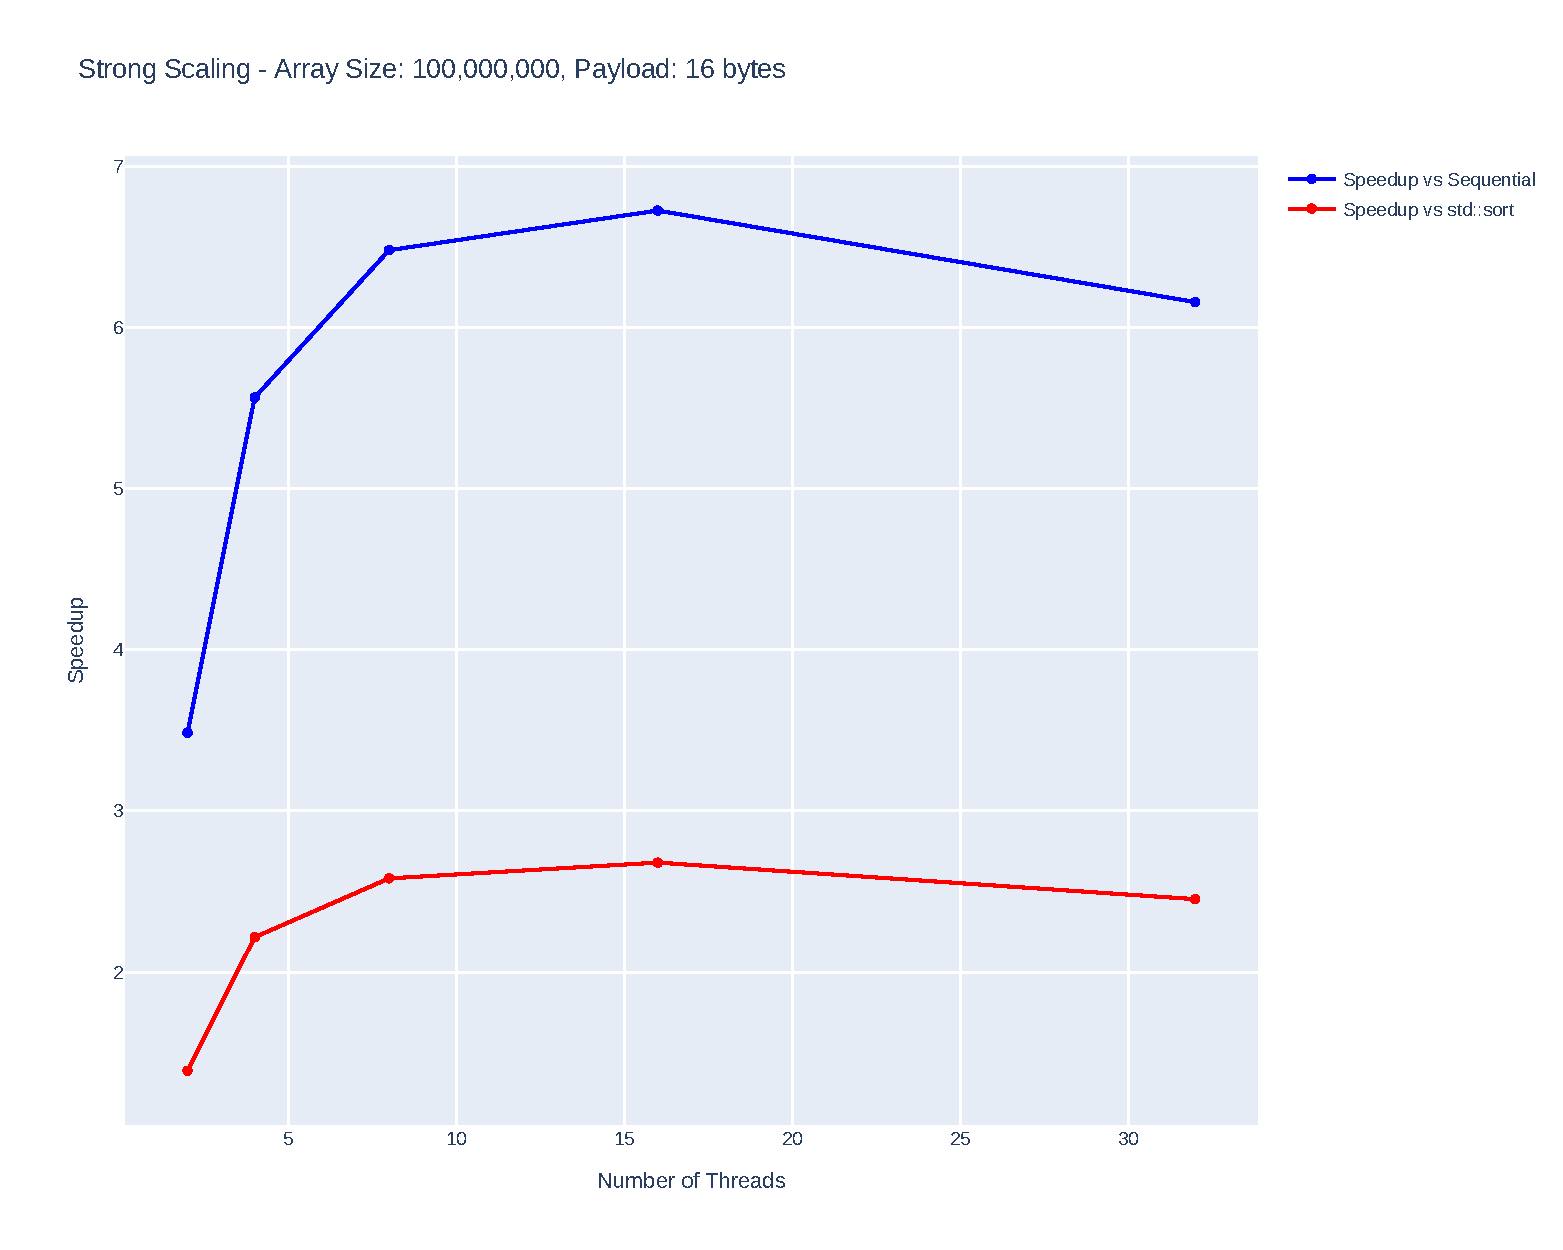
\includegraphics[width=\linewidth]{../python/plots/strong_scaling.pdf}
        \caption{Strong scaling on a single node (100M records).}
        \label{fig:strong_scaling}
    \end{subfigure}
    \hfill
    \begin{subfigure}{0.49\textwidth}
        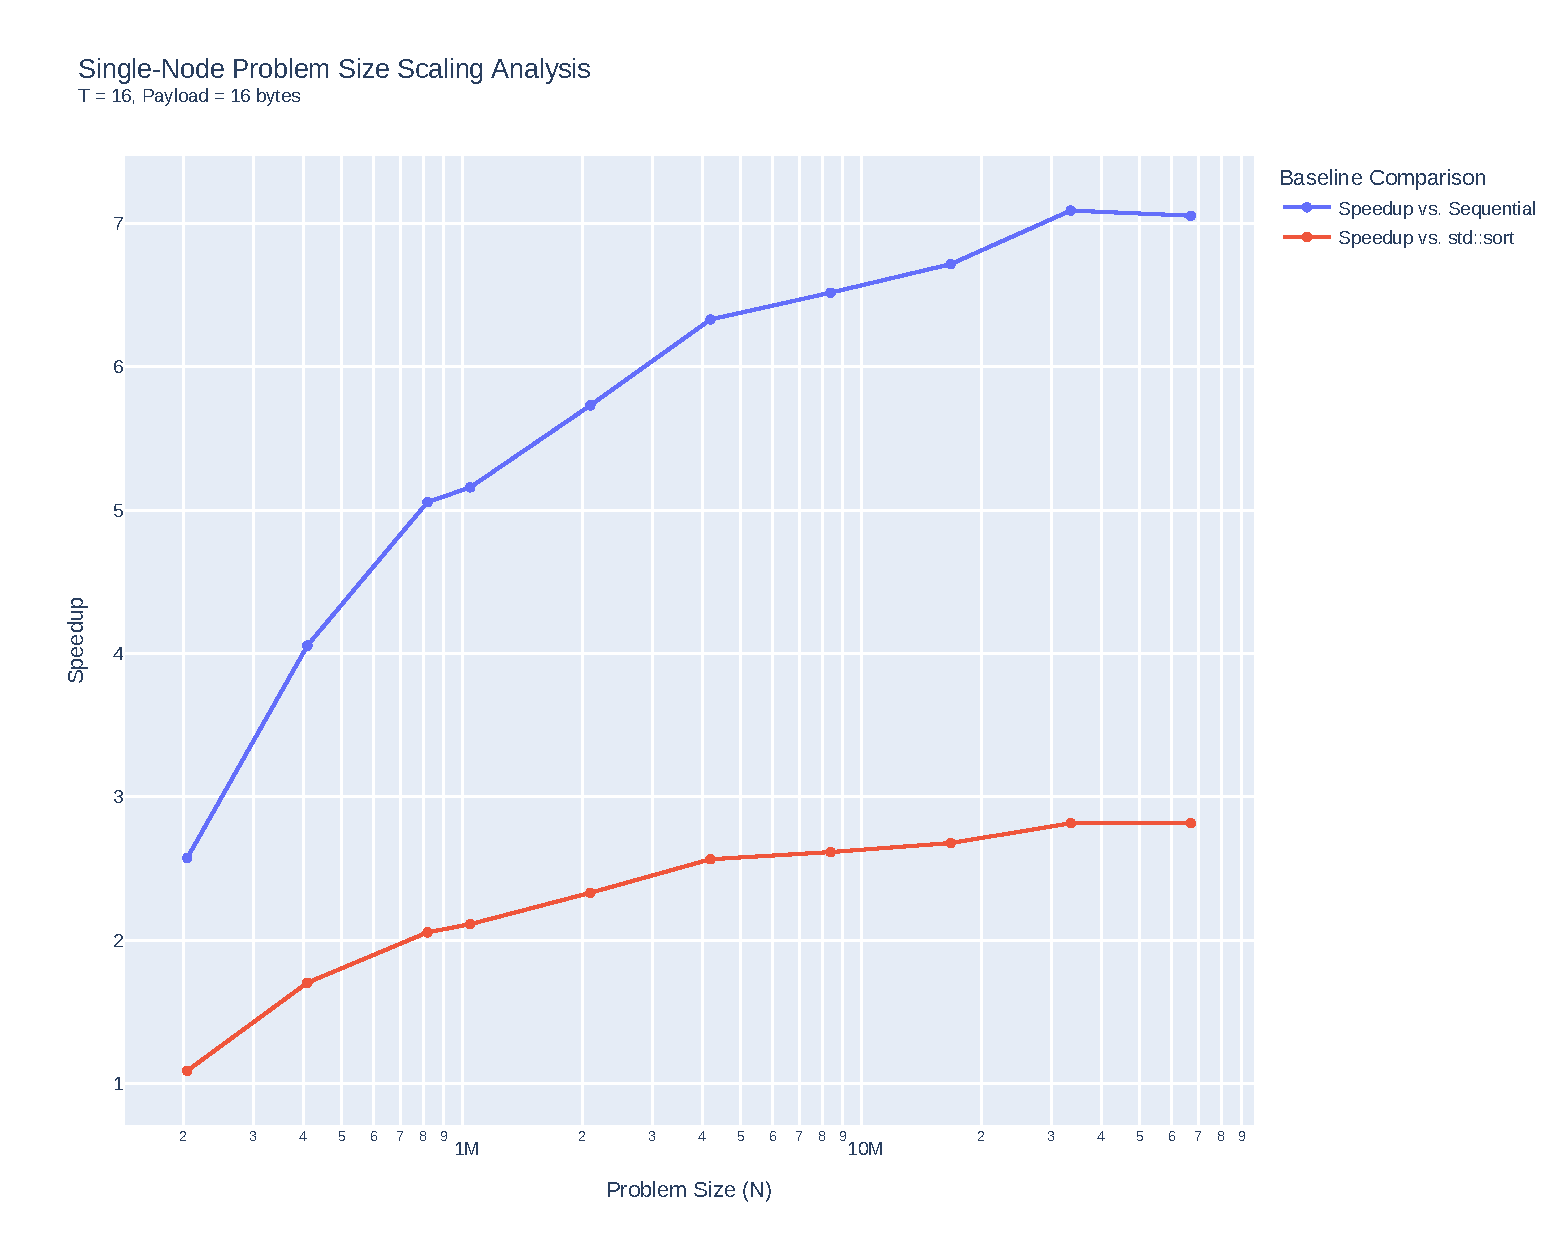
\includegraphics[width=\linewidth]{../python/plots/weak_scaling.pdf}
        \caption{Weak scaling on a single node (fixed 16 threads).}
        \label{fig:weak_scaling}
    \end{subfigure}
    \caption{Single-node performance analysis. Speedup is relative to our sequential MergeSort and the standard library's \code{std::sort}.}
    \label{fig:scaling_single_node}
\end{figure}

\textbf{Single-Node Strong Scaling.} Figure \ref{fig:strong_scaling} shows the strong scaling of our FastFlow implementation. The speedup increases significantly up to 16 threads, reaching a peak of approximately 6.8x against our sequential implementation and 2.7x against \code{std::sort}. Beyond 16 threads, performance begins to degrade. This behavior is expected and illustrates a more realistic version of Amdahl's Law, where parallel overhead is not negligible. As more threads are added, the overhead of synchronization, thread management, and contention on the memory bus starts to dominate the gains from parallel computation. The curve suggests that for this problem size and hardware, 16 threads is near the optimal point of diminishing returns.

\textbf{Single-Node Weak Scaling.} Figure \ref{fig:weak_scaling} presents a weak scaling analysis where the number of threads is fixed at 16, and the total problem size is increased. The speedup continues to grow almost linearly with the problem size. This aligns with Gustafson's Law: by increasing the problem size along with the computational resources, the serial fraction of the work becomes less significant, and the performance scales well. With more data to process, the initial costs of setting up farms and threads are amortized over a longer execution time, leading to better efficiency.

\begin{figure}[H]
    \centering
    \begin{subfigure}{0.49\textwidth}
        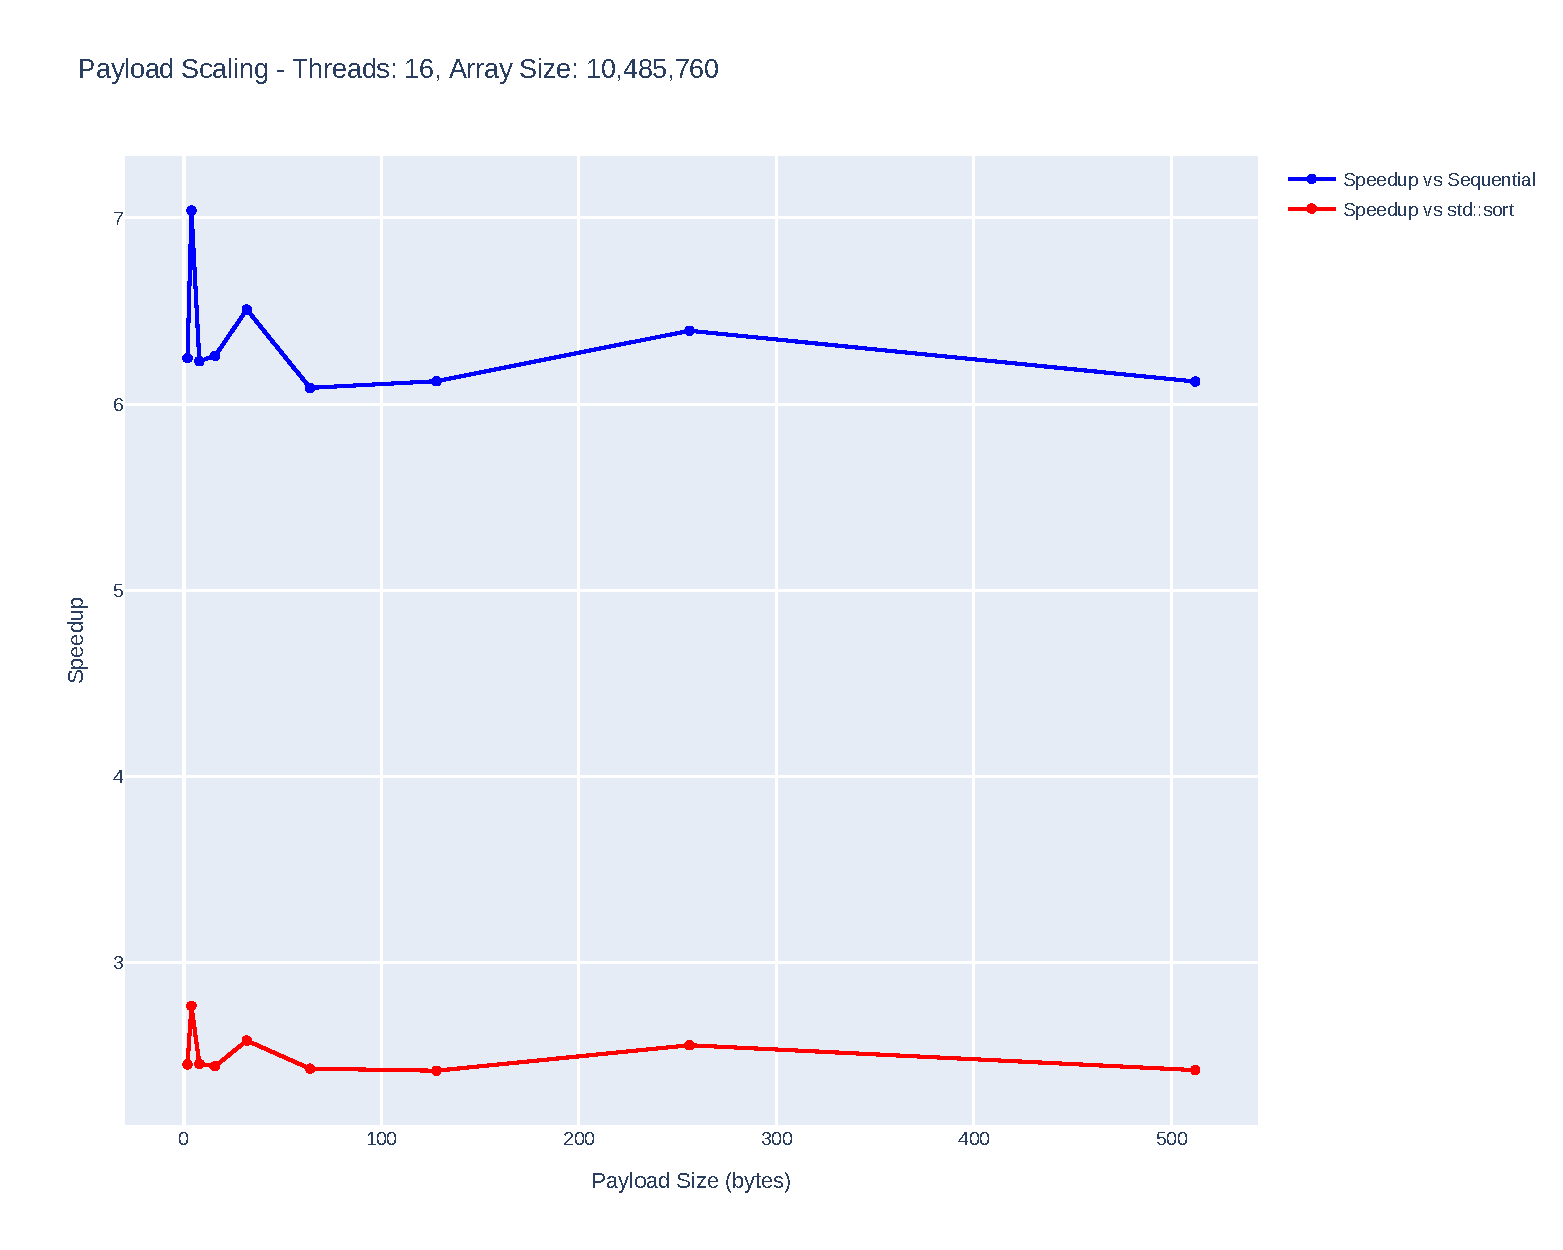
\includegraphics[width=\linewidth]{../python/plots/payload_scaling.pdf}
        \caption{Impact of record payload size (10M records).}
        \label{fig:payload_scaling}
    \end{subfigure}
    \hfill
    \begin{subfigure}{0.49\textwidth}
        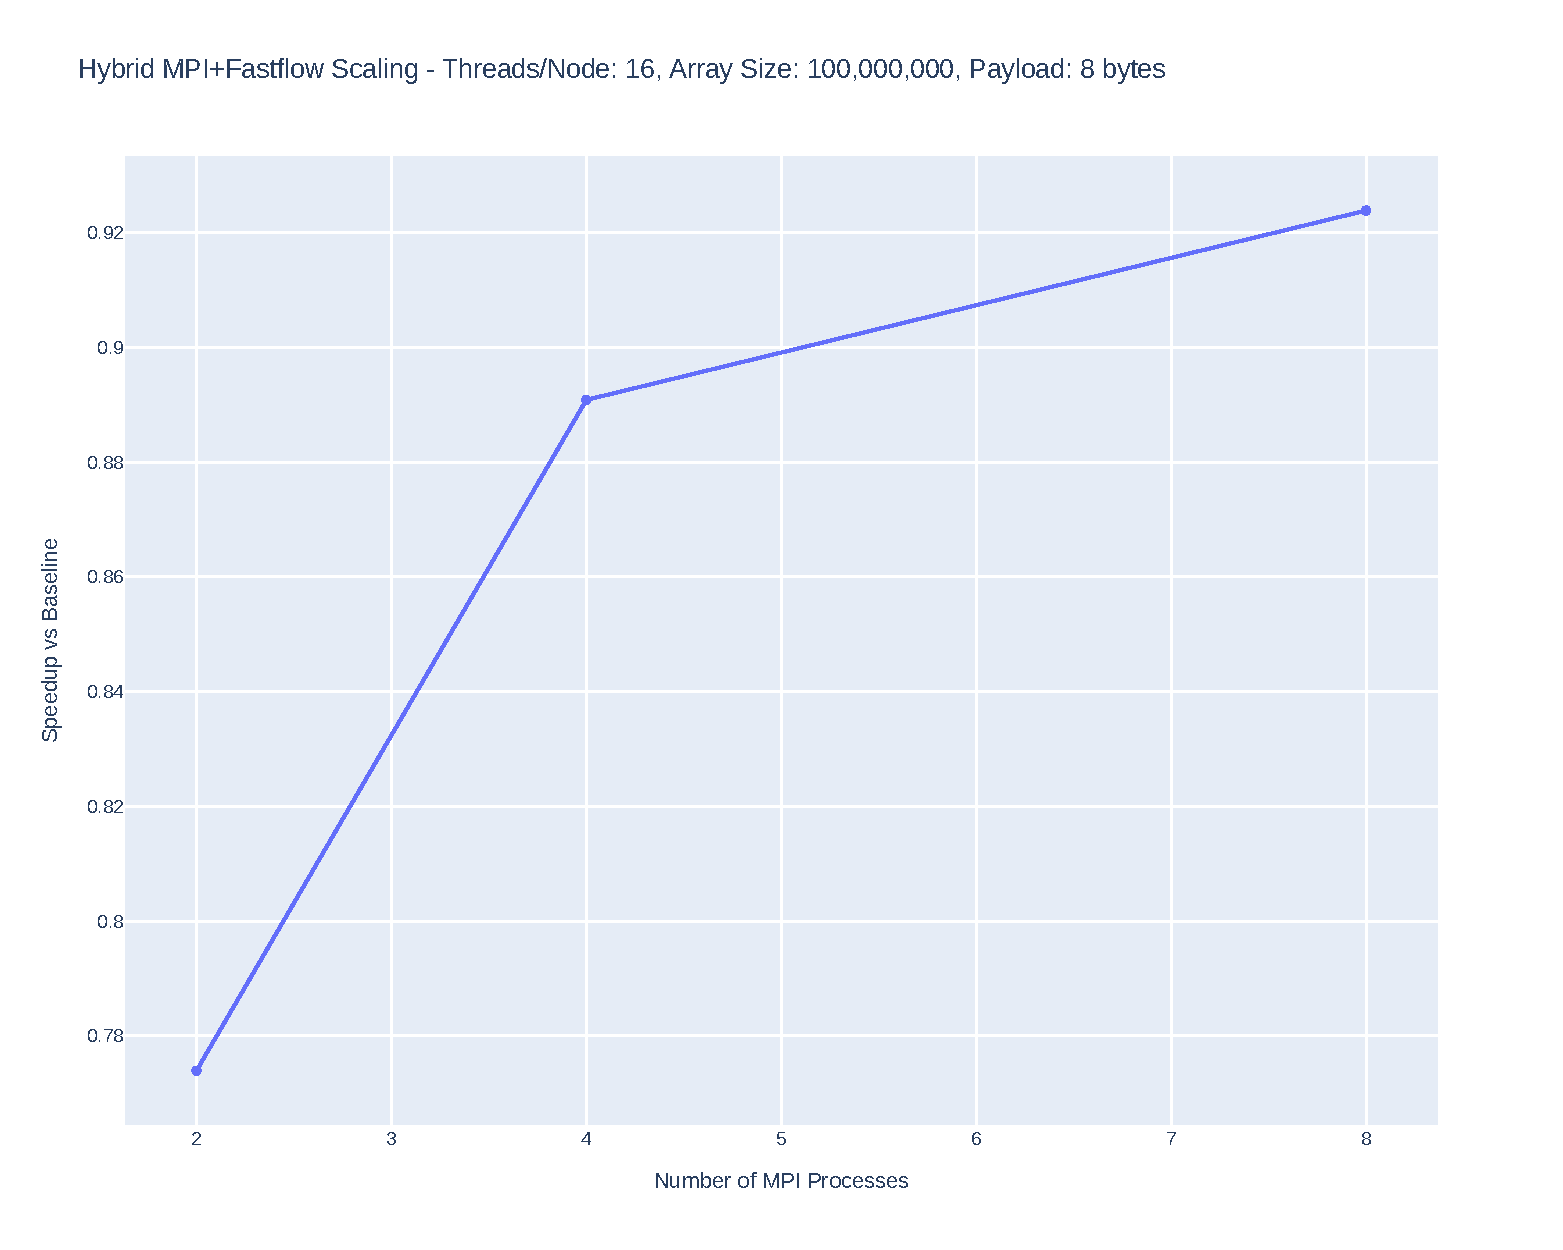
\includegraphics[width=\linewidth]{../python/plots/cluster_scaling.pdf}
        \caption{Hybrid MPI+FastFlow scaling vs. single-node baseline.}
        \label{fig:cluster_scaling}
    \end{subfigure}
    \caption{Payload and multi-node scaling analysis.}
    \label{fig:scaling_cluster}
\end{figure}

\textbf{Payload Scaling.} The impact of payload size is shown in Figure \ref{fig:payload_scaling}. The speedup is somewhat volatile for very small payloads but remains relatively stable for payloads from 8 to 512 bytes. This indicates that the algorithm's performance is heavily influenced by memory bandwidth. The primary cost in the merge phase is moving data, and this cost scales linearly with the record size. For very small payloads, the algorithm may be more sensitive to memory latency and cache effects, explaining the initial volatility. As the payload grows, the problem becomes firmly memory-bandwidth bound, as the time spent in computation (key comparisons) becomes negligible compared to the time spent in \code{std::move}.

\textbf{Hybrid MPI Scaling and Communication Overhead.} Figure \ref{fig:cluster_scaling} provides an instructive view into the performance characteristics of the hybrid algorithm. The y-axis shows speedup relative to the optimized single-node parallel baseline (1 MPI process with 16 threads). The results show that while the two-process run is slower due to initial communication overhead, the hybrid implementation achieves a positive speedup with four and eight processes. This demonstrates that for a sufficiently large problem size, distributing the computational load across multiple nodes can effectively overcome the high cost of network communication. The primary sources of overhead remain the initial data distribution via \code{MPI\_Scatterv} and the subsequent transmission of sorted partitions during the hierarchical merge. However, the performance data indicates that the time saved by parallelizing the local sort and the initial merge steps across multiple nodes is greater than the time spent on network transfers, once a certain threshold of parallelism is reached. The diminishing returns in efficiency as more nodes are added are expected, following Amdahl's law, as communication and synchronization costs begin to represent a larger fraction of the total execution time. Achieving a positive speedup confirms the viability of the hybrid approach for large-scale datasets.


\end{document}
